\chapter{Arhitektura i dizajn sustava}
	
	\justify{Arhitektura se može podijeliti na sljedeće podsustave:}
	\begin{itemize}
		\item Mobilni uređaj
		\item Mobilna aplikacija
		\item Baza podataka	
	\end{itemize}

	\begin{figure}[h]
		\centering
		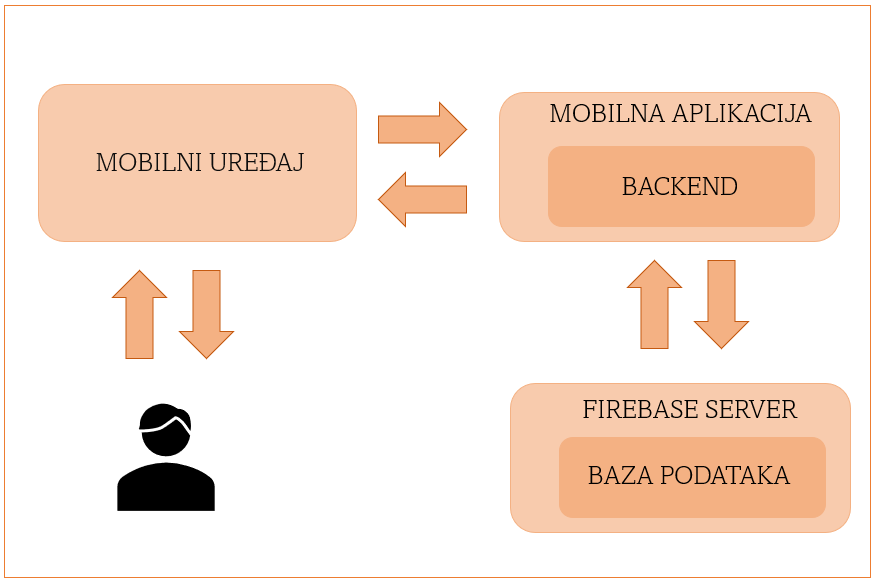
\includegraphics[width=\textwidth]{Arhitektura.png}
		\caption{Arhitektura sustava}
	\end{figure}

	\justify{\textbf{Mobilni (Android) uređaj} je uređaj koji korisniku omogućuje pokretanje Android mobilne aplikacije. Aplikacija je napisana u kodu te nakon toga uređaj taj kod interpretira i prikazuje ga korisniku kao grafičko sučelje. Pomoću uređaja
	korisnik ineraktira s aplikacijom i preko nje šalje upite bazi podataka.}

	\justify{\textbf{Mobilna aplikacija} je glavni dio arhitekture. Korisnik istu koristi kako bi obradio svoje zahtjeve. Ona se sastoji od \textit{Frontend} i \textit{Backend} dijela te pomoću \textit{Backenda} komunicira s bazom podataka, čitajući ili pišući podatke u nju. Nakon toga se korisniku preko \textit{Frontend} dijela
	prikazuju potrebni podaci.}

	Programski jezik koji smo koristili za izradu naše mobilne je Kotlin, koji je Google 2019. proglasio kao preferirani jezik izrade Android aplikacija. Razvojno okruženje
	s najboljom podrškom za izradu takvih aplikacija je Android Studio, koji smo i mi upotrebljavali. Jedan dio \textit{Backend} programskog koda napisan je u JavaScript programskom jeziku, 
	u Node.js okruženju. Arhitektura sustava se temelji na MVVM (Model-View-Viewmodel) konceptu, koji je dio svake Android aplikacije.

	Odlika MVVM-a je što pomaže organizirati kod i podijeliti program u manje dijelove kako bi razvoj, ažuriranje i ponovna upotreba koda bila jednostavnija i brža.
	MVVM se sastoji od:
	\begin{itemize}
		\item \textbf{Model} - odnosi se ili na model domene, koji predstavlja sadržaj stvarnog stanja (objektno orijentirani pristup), ili na sloj pristupa podacima, koji predstavlja sadržaj.
		\item \textbf{View} - struktura, raspored i izgled onoga što korisnik vidi na zaslonu. Prikazuje model i 
		prima interakciju korisnika s prikazom (klikovi mišem, unos tipkovnice, dodirivanja zaslona, itd.).
		\item \textbf{Viewmodel} - nalazi se između Viewa i Modela. Ovdje su smještene kontrole za interakciju s Viewom, dok se \textit{binding} koristi za povezivanje elemenata korisničkog sučelja
		 u Viewu s kontrolama u ViewModelu.
	\end{itemize}
	
				
		\section{Baza podataka}
			
		\justifying{Za potrebe našeg sustava koristit ćemo nerelacijsku bazu podataka (NoSQL) ugrađenu u Firebase alat koji olakšava rad s podatcima. Firebase nudi nekoliko vrsta baza, a mi smo izabrali Firestore verziju. Baza se sastoji od nekoliko kolekcija koja se definira imenom i skupom dokumenata, a svaki dokument ima svoje atribute. Atributi se sastoje od imena, tipa podataka i samog podatka. Temelje se na modelu ključ-vrijednost. Kako svaki dokument unutar kolekcije može imati različite atribute, važno je održati konzistentnost podataka, baza mora biti dosljedna i to se postiže kreiranjem modela unutar aplikacije. Na taj način će svi dokumenti unutar kolekcije imati iste atribute.
		Baza se sastoji od sljedećih kolekcija: 
		}
		\begin{itemize}
			\item documentArchive
			\item documentStatus
			\item documentByUser
			\item documents 
			\item users
			\item tokens
		\end{itemize}
		
			\subsection{Opis tablica}
			

			\justify{\textit{\textbf{Napomena:} Iz razloga što se u službenoj Firebase dokumentaciji koriste izrazi collection i document te zato što se naša aplikacija bavi skeniranjem dokumenata, može doći do zabune kad je koji izraz za dokument upotrijebljen (Firebaseov ili iz aplikacije). Stoga će se u daljnjem tekstu za izraz koji se odnosi na fizičke (skenirane) dokumente koristiti riječ \textbf{dokument}, a za Firebaseov član kolekcije riječ \textbf{document}.}}

			\justify{\textbf{documentArchive}   Ova kolekcija sadrži informaciju o arhiviranju dokumenata. Dokumentu koji je arhiviran, tj. spremljen u bazu, se automatski generira identifikator te \textit{documenti} u \textit{documentArchive} kolekciji dobivaju iste te identifikatore, kako bi se znalo za koji skenirani dokument sadrži podatke. Kolekcija se sastoji od atributa \textit{archiveId} i \textit{archivedOn}, koji govori vrijeme kreiranja arhive. Svakom \textit{documentu} iz kolekcije \textit{documents} pripada jedan \textit{document} iz kolekcije \textit{documentArchive}.}
			
				\begin{longtblr}[
					label=none,
					entry=none
					]{
						width = \textwidth,
						colspec={|X[6,l]|X[6, l]|X[20, l]|}, 
						rowhead = 1,
					} %definicija širine tablice, širine stupaca, poravnanje i broja redaka naslova tablice
					\hline \multicolumn{3}{|c|}{\textbf{documentArchive}}	 \\ \hline[3pt]
					\SetCell{LightGreen}documentId & string	&  	Jedinstveni identifikator arhive. Jednak id-u dokumenta koji je arhiviran\\ \hline
					archiveId	& string &   	\\ \hline 
					archivedOn  & timestamp & datum i vrijeme arhiviranja dokumenta   \\ \hline
				\end{longtblr}


			\justify{\textbf{documentStatus}  Ova se kolekcija sastoji od nekoliko atributa vezanih za status dokumenta. Sadrži atribute \textit{archived, revised, scannedProperly, toBeSigned, signed}. Primjerice, nakon što se dokument uspješno skenira, vrijednosti \textit{archived, scannedProperly} i \textit{toBeSigned} se postavljaju na \textit{true}. U slučaju da u aplikaciji treba filtrirati dokumente koji zadovoljavaju jedan ili više statusa, ova kolekcija dolazi u uporabu. Za svaki \textit{document} iz kolekcije \textit{documents} postoji jedan   \textit{document} iz ove kolekcije, s istim identifikatorom.}
				
				\begin{longtblr}[
					label=none,
					entry=none
					]{
						width = \textwidth,
						colspec={|X[10,l]|X[6, l]|X[20, l]|}, 
						rowhead = 1,
					} %definicija širine tablice, širine stupaca, poravnanje i broja redaka naslova tablice
					\hline \multicolumn{3}{|c|}{\textbf{documentStatus}}	 \\ \hline[3pt]
					\SetCell{LightBlue}documentId & string	&  	Jedinstveni identifikator. Jednak id-u dokumenta koji je skeniran\\ \hline
					archived	& boolean &  oznaka je li dokument arhiviran 	\\ \hline 
					revised  & boolean & oznaka je li dokument reviziran   \\ \hline
					scannedProperly  & boolean & oznaka je li dokument pravilno skeniran   \\ \hline
					signed  & boolean & oznaka je li dokument potpisan   \\ \hline
					toBeSigned  & boolean & oznaka je li dokument poslan na slanje   \\ \hline
					
				\end{longtblr}

				\justify{\textbf{documentByUser}  Kolekcija koja informira o detaljnijim podacima dokumenta, tj. prikazuje koji je \textit{user} napravio koji korak u protoku dokumenta kroz aplikaciju. Sadrži atribute \textit{archivedBy, revisedBy, sentToSignBy, signedBy}. U polju svakog od atributa nalazi se  id nekog \textit{usera}. Za svaki \textit{document} iz kolekcije \textit{documents} postoji jedan   \textit{document} iz ove kolekcije, s istim identifikatorom.				
				\begin{longtblr}[
					label=none,
					entry=none
					]{
						width = \textwidth,
						colspec={|X[10,l]|X[6, l]|X[20, l]|}, 
						rowhead = 1,
					} %definicija širine tablice, širine stupaca, poravnanje i broja redaka naslova tablice
					\hline \multicolumn{3}{|c|}{\textbf{documentByUser}}	 \\ \hline[3pt]
					\SetCell{LightBlue}documentId & string	&  	Jedinstveni identifikator. Jednak id-u dokumenta koji je skeniran\\ \hline
					archivedBy	& string &  id usera koji je arhivirao dokument 	\\ \hline 
					revisedBy  & boolean & id usera koji je revizirao dokument   \\ \hline
					toBeSignBy  & boolean & id usera koji je dokument poslao na potpisivanje \\ \hline
					signedBy  & boolean & id usera koji je potpisao dokument  \\ \hline
				\end{longtblr}
			

			\justify{\textbf{documents}  Kolekcija koja sadrži informacije o skeniranim dokumentima. Postoji nekoliko specijalizacija dokumenta, a to su \textbf{Račun}, \textbf{Ponuda} i \textbf{Interni dokument}. Dokumenti sadrže zajednički skup atributa, \textit{createdOn}, \textit{type}, \textit{user}, \textit{label} te svaka od specijalizacija ima svoje zasebne atribute. Svakom dokumentu se može pridružiti jedan \textit{document} iz kolekcija \textit{documentArchive}, \textit{documentStatus} i \textit{users}. Identifikator pojedinog \textit{usera} se u ovoj kolekciji sprema pod atribut \textit{user}.}
				
				\begin{longtblr}[
					label=none,
					entry=none
					]{
						width = \textwidth,
						colspec={|X[10,l]|X[6, l]|X[20, l]|}, 
						rowhead = 1,
					} %definicija širine tablice, širine stupaca, poravnanje i broja redaka naslova tablice
					\hline \multicolumn{3}{|c|}{\textbf{documents}}	 \\ \hline[3pt]
					\SetCell{LightGreen}documentId & string	&  	Jedinstveni identifikator skeniranog dokumenta\\ \hline
					createdOn  & timestamp & datum i vrijeme kreiranja dokumenta   \\ \hline
					label  & string & oznaka s dokumenta   \\ \hline
					type  & string & tip dokumenta: Račun, Ponuda, Interni dokument   \\ \hline
					user  & string & ID korisnika koji je obavio skeniranje   \\ \hline
					clientName	& string &  ime i prezime klijenta s Računa	\\ \hline 
					items  & map of numbers & artikli s Računa ili Ponude   \\ \hline
					totalPrice  & number & ukupna cijena artikala s Računa ili Ponude   \\ \hline
					content  & string & sadržaj Internog dokumenta   \\ \hline
				\end{longtblr}

			\justify{\textbf{users}  Ova kolekcija sadrži informacije o korisnicima aplikacije koji su registrirani. Pri prvoj uporabi aplikacije svaki korisnik mora proći registraciju. U kolekciji se pohranjuju korisnikov email, ime, prezime i uloga. Korisnik može biti Direktor, Računovođa, Revizor ili Zaposlenik. Svoju ulogu korisnik odabire pri registraciji. Svaki korisnik ima svoj ID i on se sprema u kolekciju \textit{documents}, kako bi se znalo koji korisnik je skenirao koji dokument.}
				
				\begin{longtblr}[
					label=none,
					entry=none
					]{
						width = \textwidth,
						colspec={|X[6,l]|X[6, l]|X[20, l]|}, 
						rowhead = 1,
					} %definicija širine tablice, širine stupaca, poravnanje i broja redaka naslova tablice
					\hline \multicolumn{3}{|c|}{\textbf{users}}	 \\ \hline[3pt]
					\SetCell{LightGreen}documentId & string	&  	Jedinstveni identifikator registriranog korisnika\\ \hline
					email  & string & email adresa korisnika   \\ \hline
					firstName  & string & ime korisnika  \\ \hline
					lastName  & string & prezime korisnika   \\ \hline
					role  & string & uloga korisnika   \\ \hline
					specialization  & string & opcionalna specijalizacija Računovođe   \\ \hline
					
				\end{longtblr}	

			\justify{\textbf{tokens} Kolekcija s \textit{Firebase Cloud Messaging} tokenima. Ona omogućava slanje notifikacijama onim tokenima koji su u tom trenutku aktivni ili zadovoljavaju određene uvjete. Sastoji se od samo jednog atributa, \textit{token}, a jedinstveni identifikator tokena je jednak identifikatoru jednom \textit{documentu} iz kolekcije \textit{users}.}

				\begin{longtblr}[
					label=none,
					entry=none
					]{
						width = \textwidth,
						colspec={|X[6,l]|X[6, l]|X[20, l]|}, 
						rowhead = 1,
					} %definicija širine tablice, širine stupaca, poravnanje i broja redaka naslova tablice
					\hline \multicolumn{3}{|c|}{\textbf{tokens}}	 \\ \hline[3pt]
					\SetCell{LightBlue}documentId & string	&  	Jedinstveni identifikator tokena. Jednak id-u usera kojem pripada.\\ \hline
					token & string & Identifikator dodijeljen od \textit{Firebase Cloud Messaginga} \\ \hline
					
				\end{longtblr}	
			
			\subsection{Dijagram baze podataka}
			\begin{figure}[h]
				\centering
				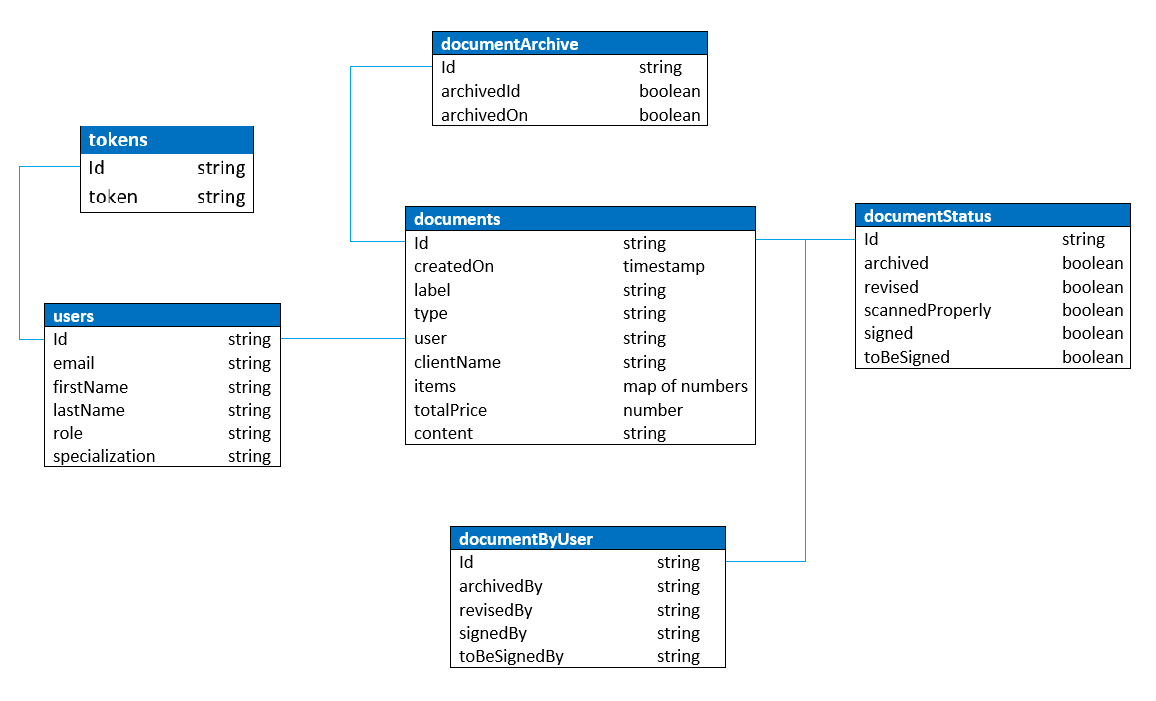
\includegraphics[width=\textwidth]{dijagramBaze.png}
				\caption{Dijagram baze podataka sustava}
			\end{figure}
			
			\eject
			
			
		\section{Dijagram razreda}
		
			\justify{Na slikama 4.3., 4.4., 4.5., 4.6. prikazani su razredi koji pripadaju MVVM arhitekturi. Zbog lakše organizacije, razredi su podijeljeni prema arhitekturi, kako bi se smanjila prenapučenost unutar dijagrama. Iz naziva i tipova podataka može se zaključiti vrsta ovisnosti između razreda.}\\
			
				
			\justify{Razredi prikazani na slici 4.3. nasljeđuju Activity i Fragment razred. Metode implementirane u tim razredima manipuliraju objektima dobivenim iz razreda sa slike 4.4. (ViewModel) te omogućuju prikaz podataka.}\\
			
			\begin{figure}[H]
				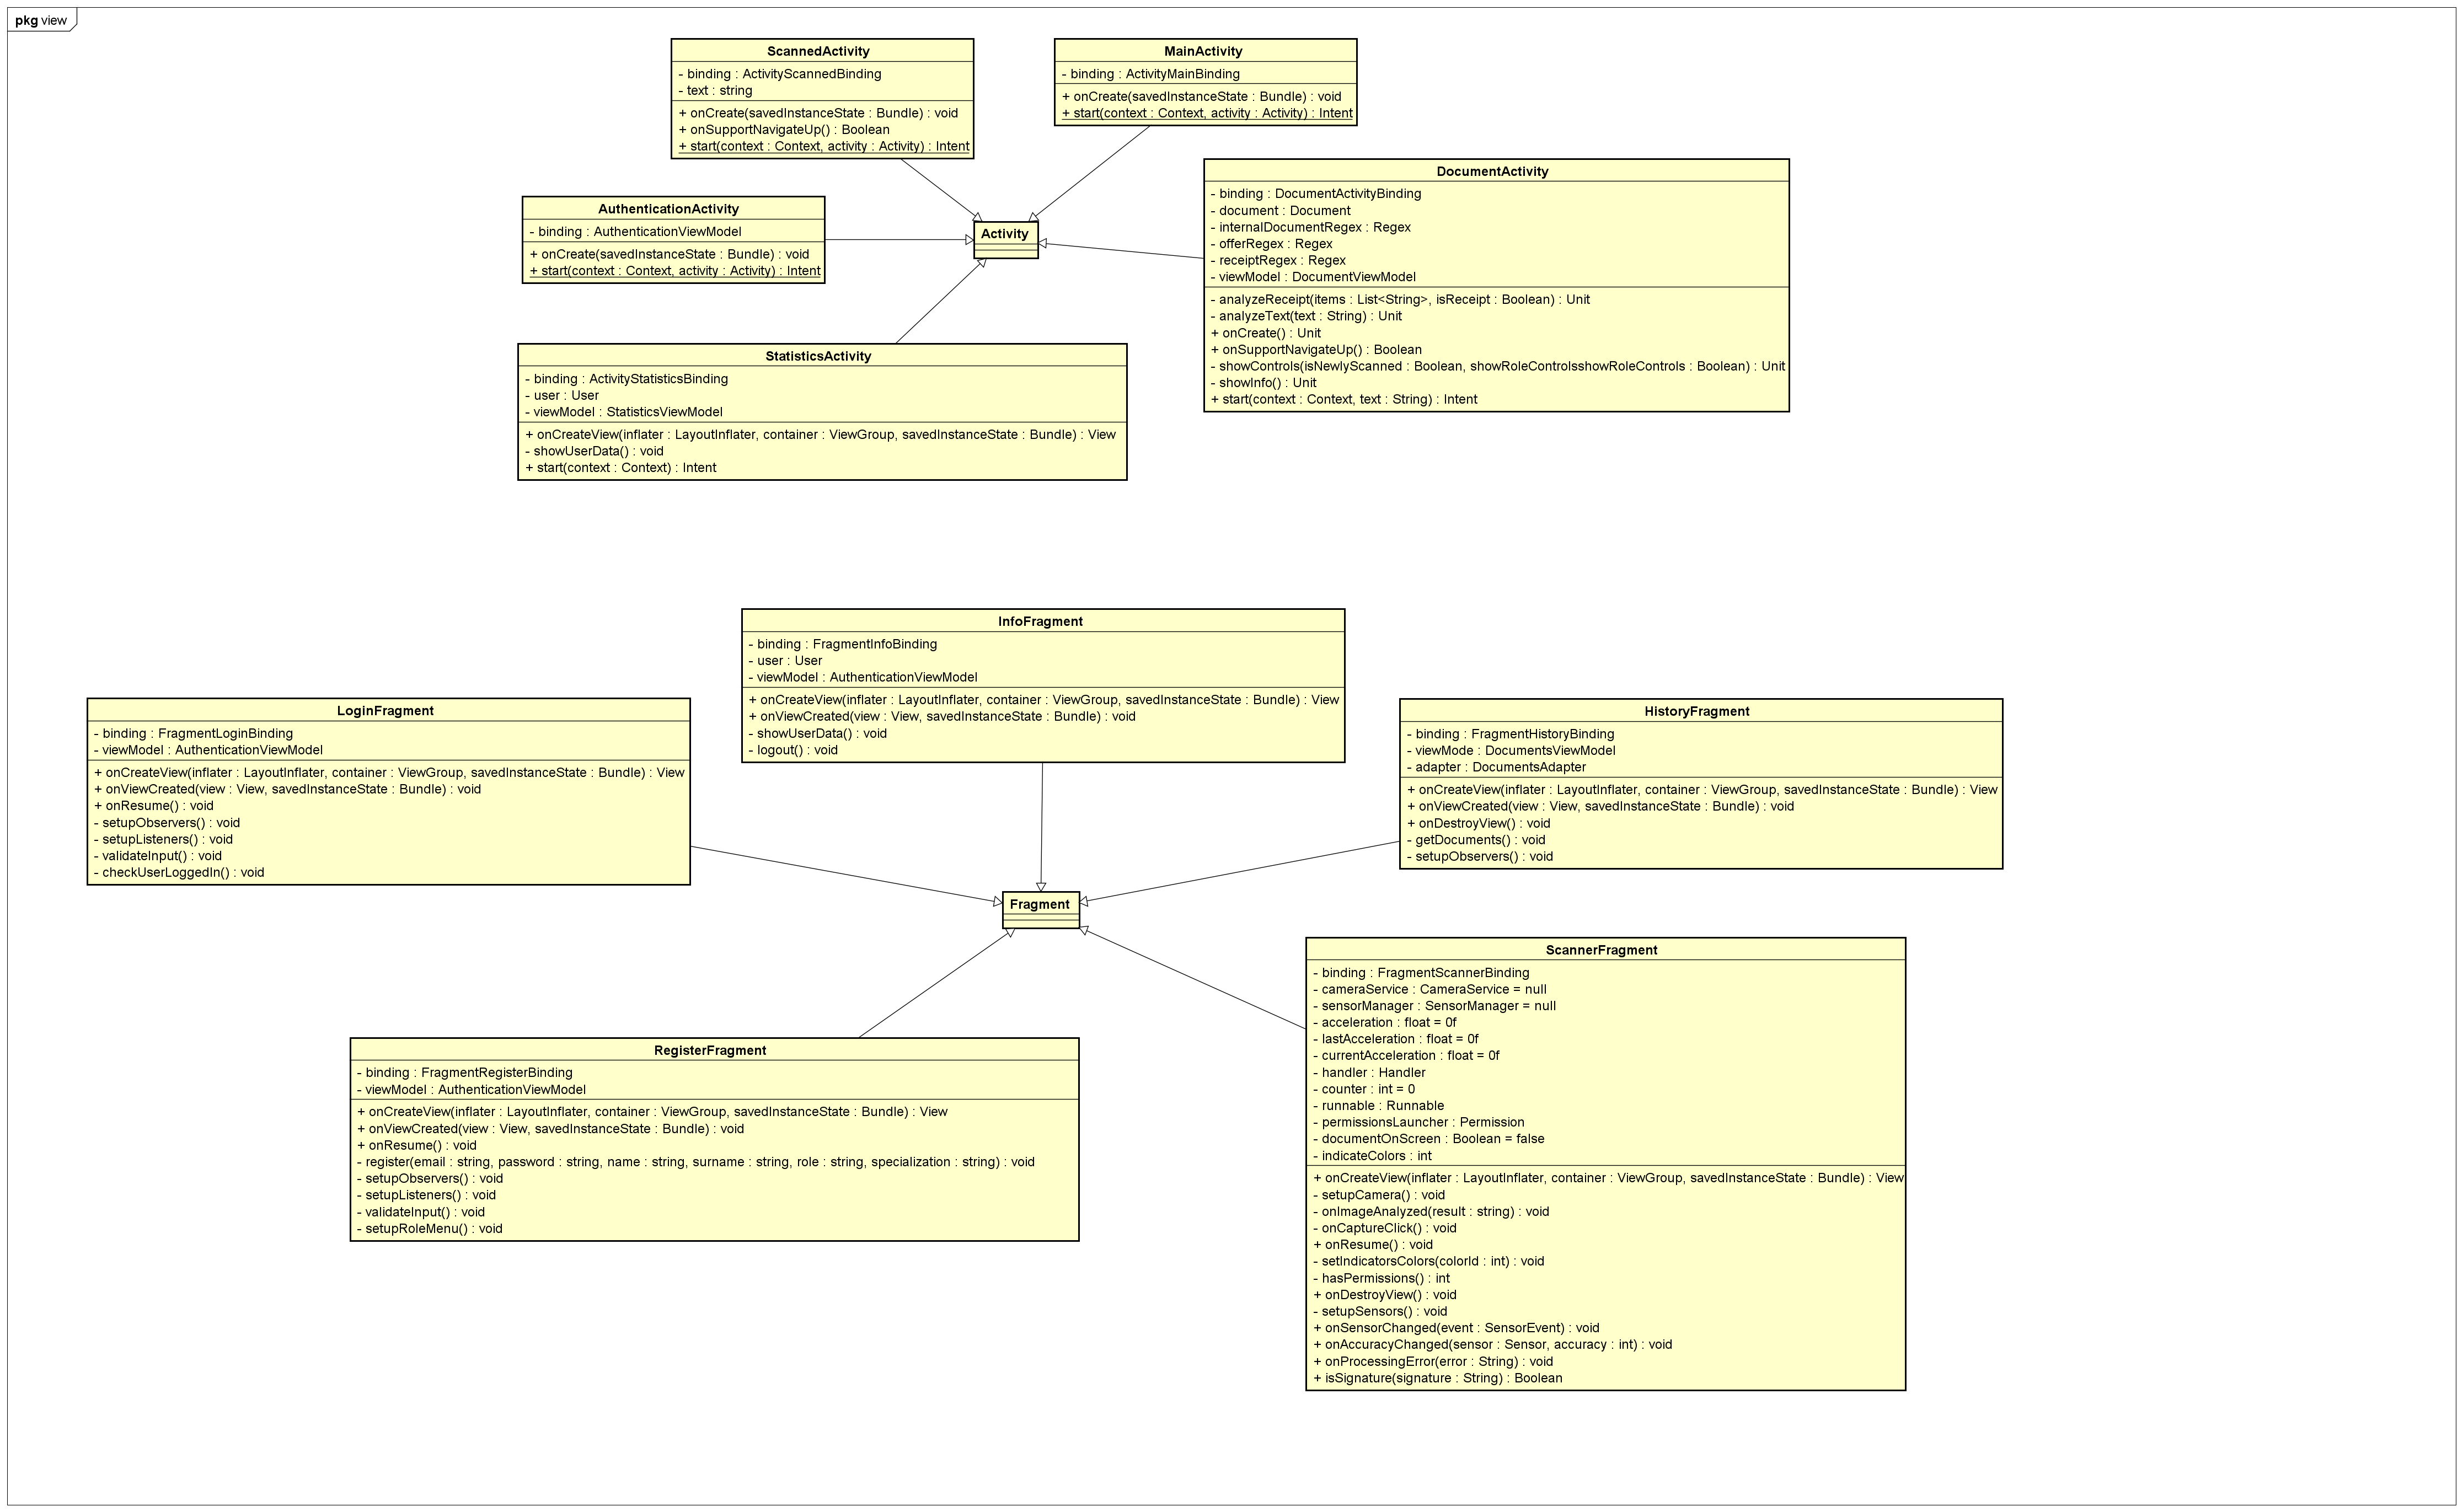
\includegraphics[width=\textwidth]{slike/Dijagram_razreda_view.png}
				\caption{Dijagram razreda - View.}
			\end{figure}
		
			\justify{Razredi DocumentsViewModel i AuthenticationViewModel uzimaju željene podatke preko razreda DocumentRepository i AuthenticationRepository, koji su direktno povezani s bazom podataka. AuthenticationRepository razred koristi se razredom AuthHelper kako bi prilikom registracije stvorio novog korisnika, a DocumentRepository koristi se razredom DocumentsHelper kako bi omogućio stvaranje dokumenata. Način na koji su povezani razredi iz view i viewModel dijela arhitekture prikazani su na slici 4.5.}\\
					
			\begin{figure}[H]
				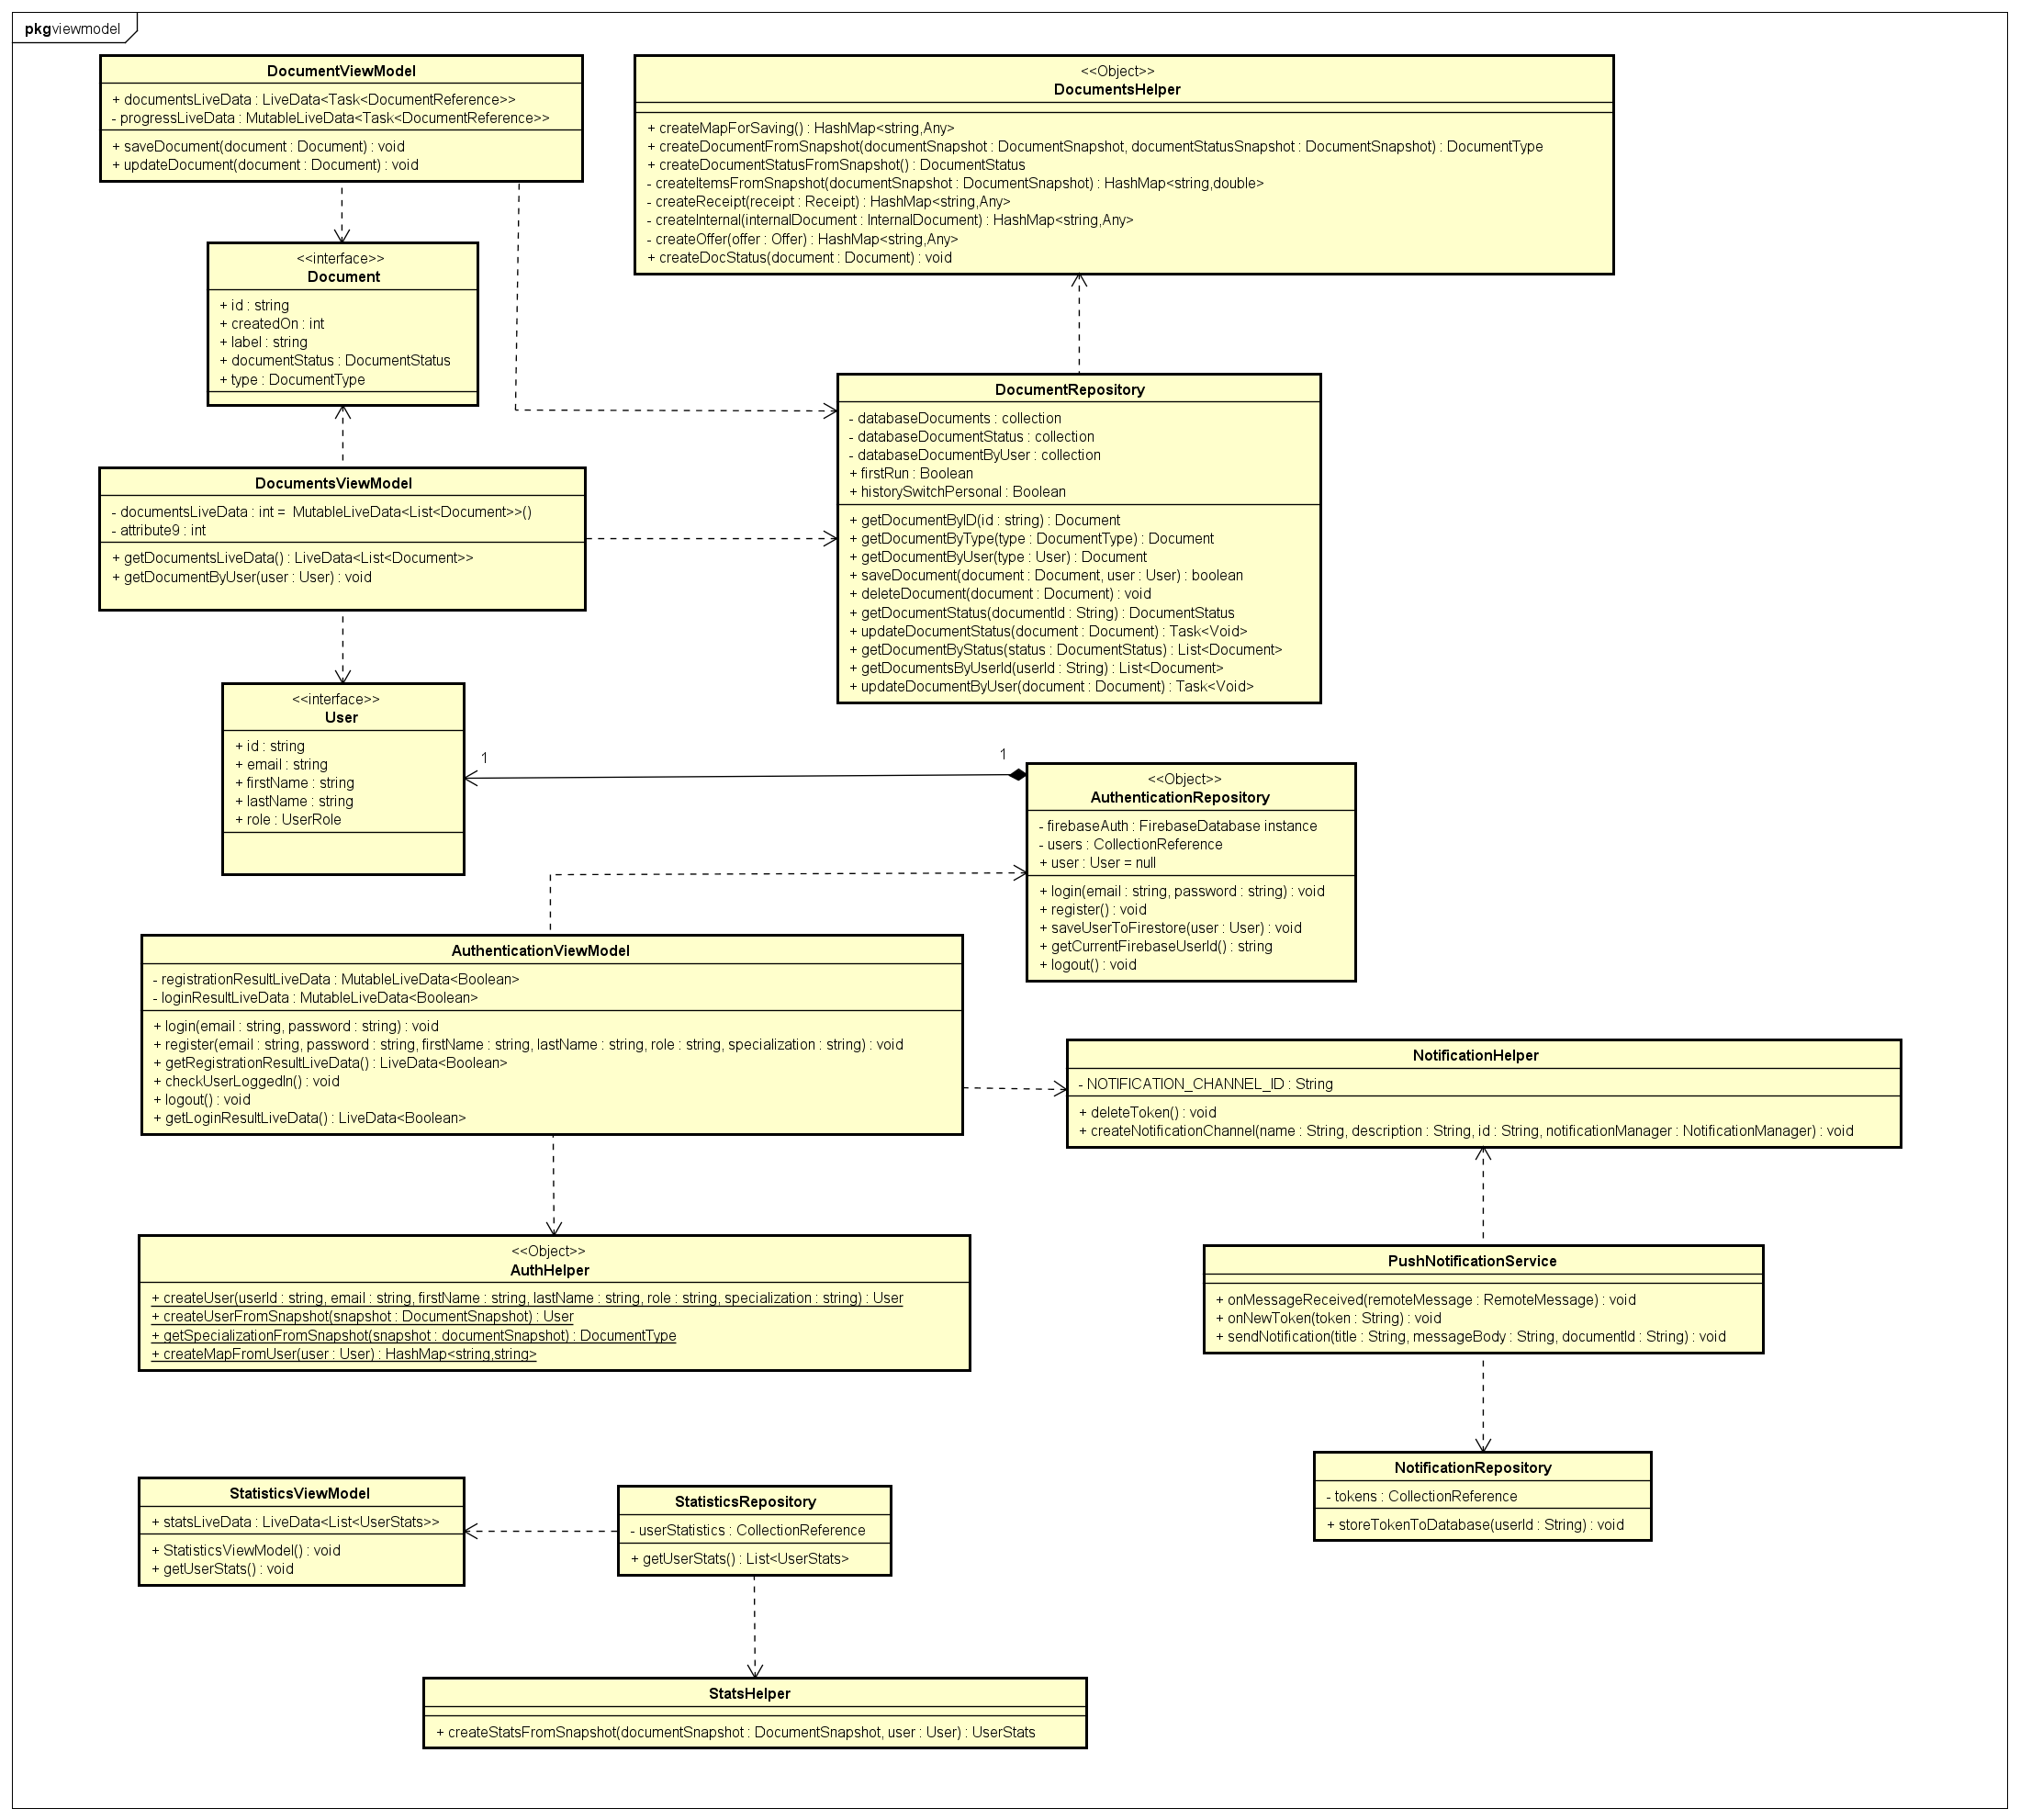
\includegraphics[width=\textwidth]{slike/Dijagram_razreda_viewModel.png}
				\caption{Dijagram razreda - ViewModel.}
			\end{figure}
		
			\begin{figure}[H]
				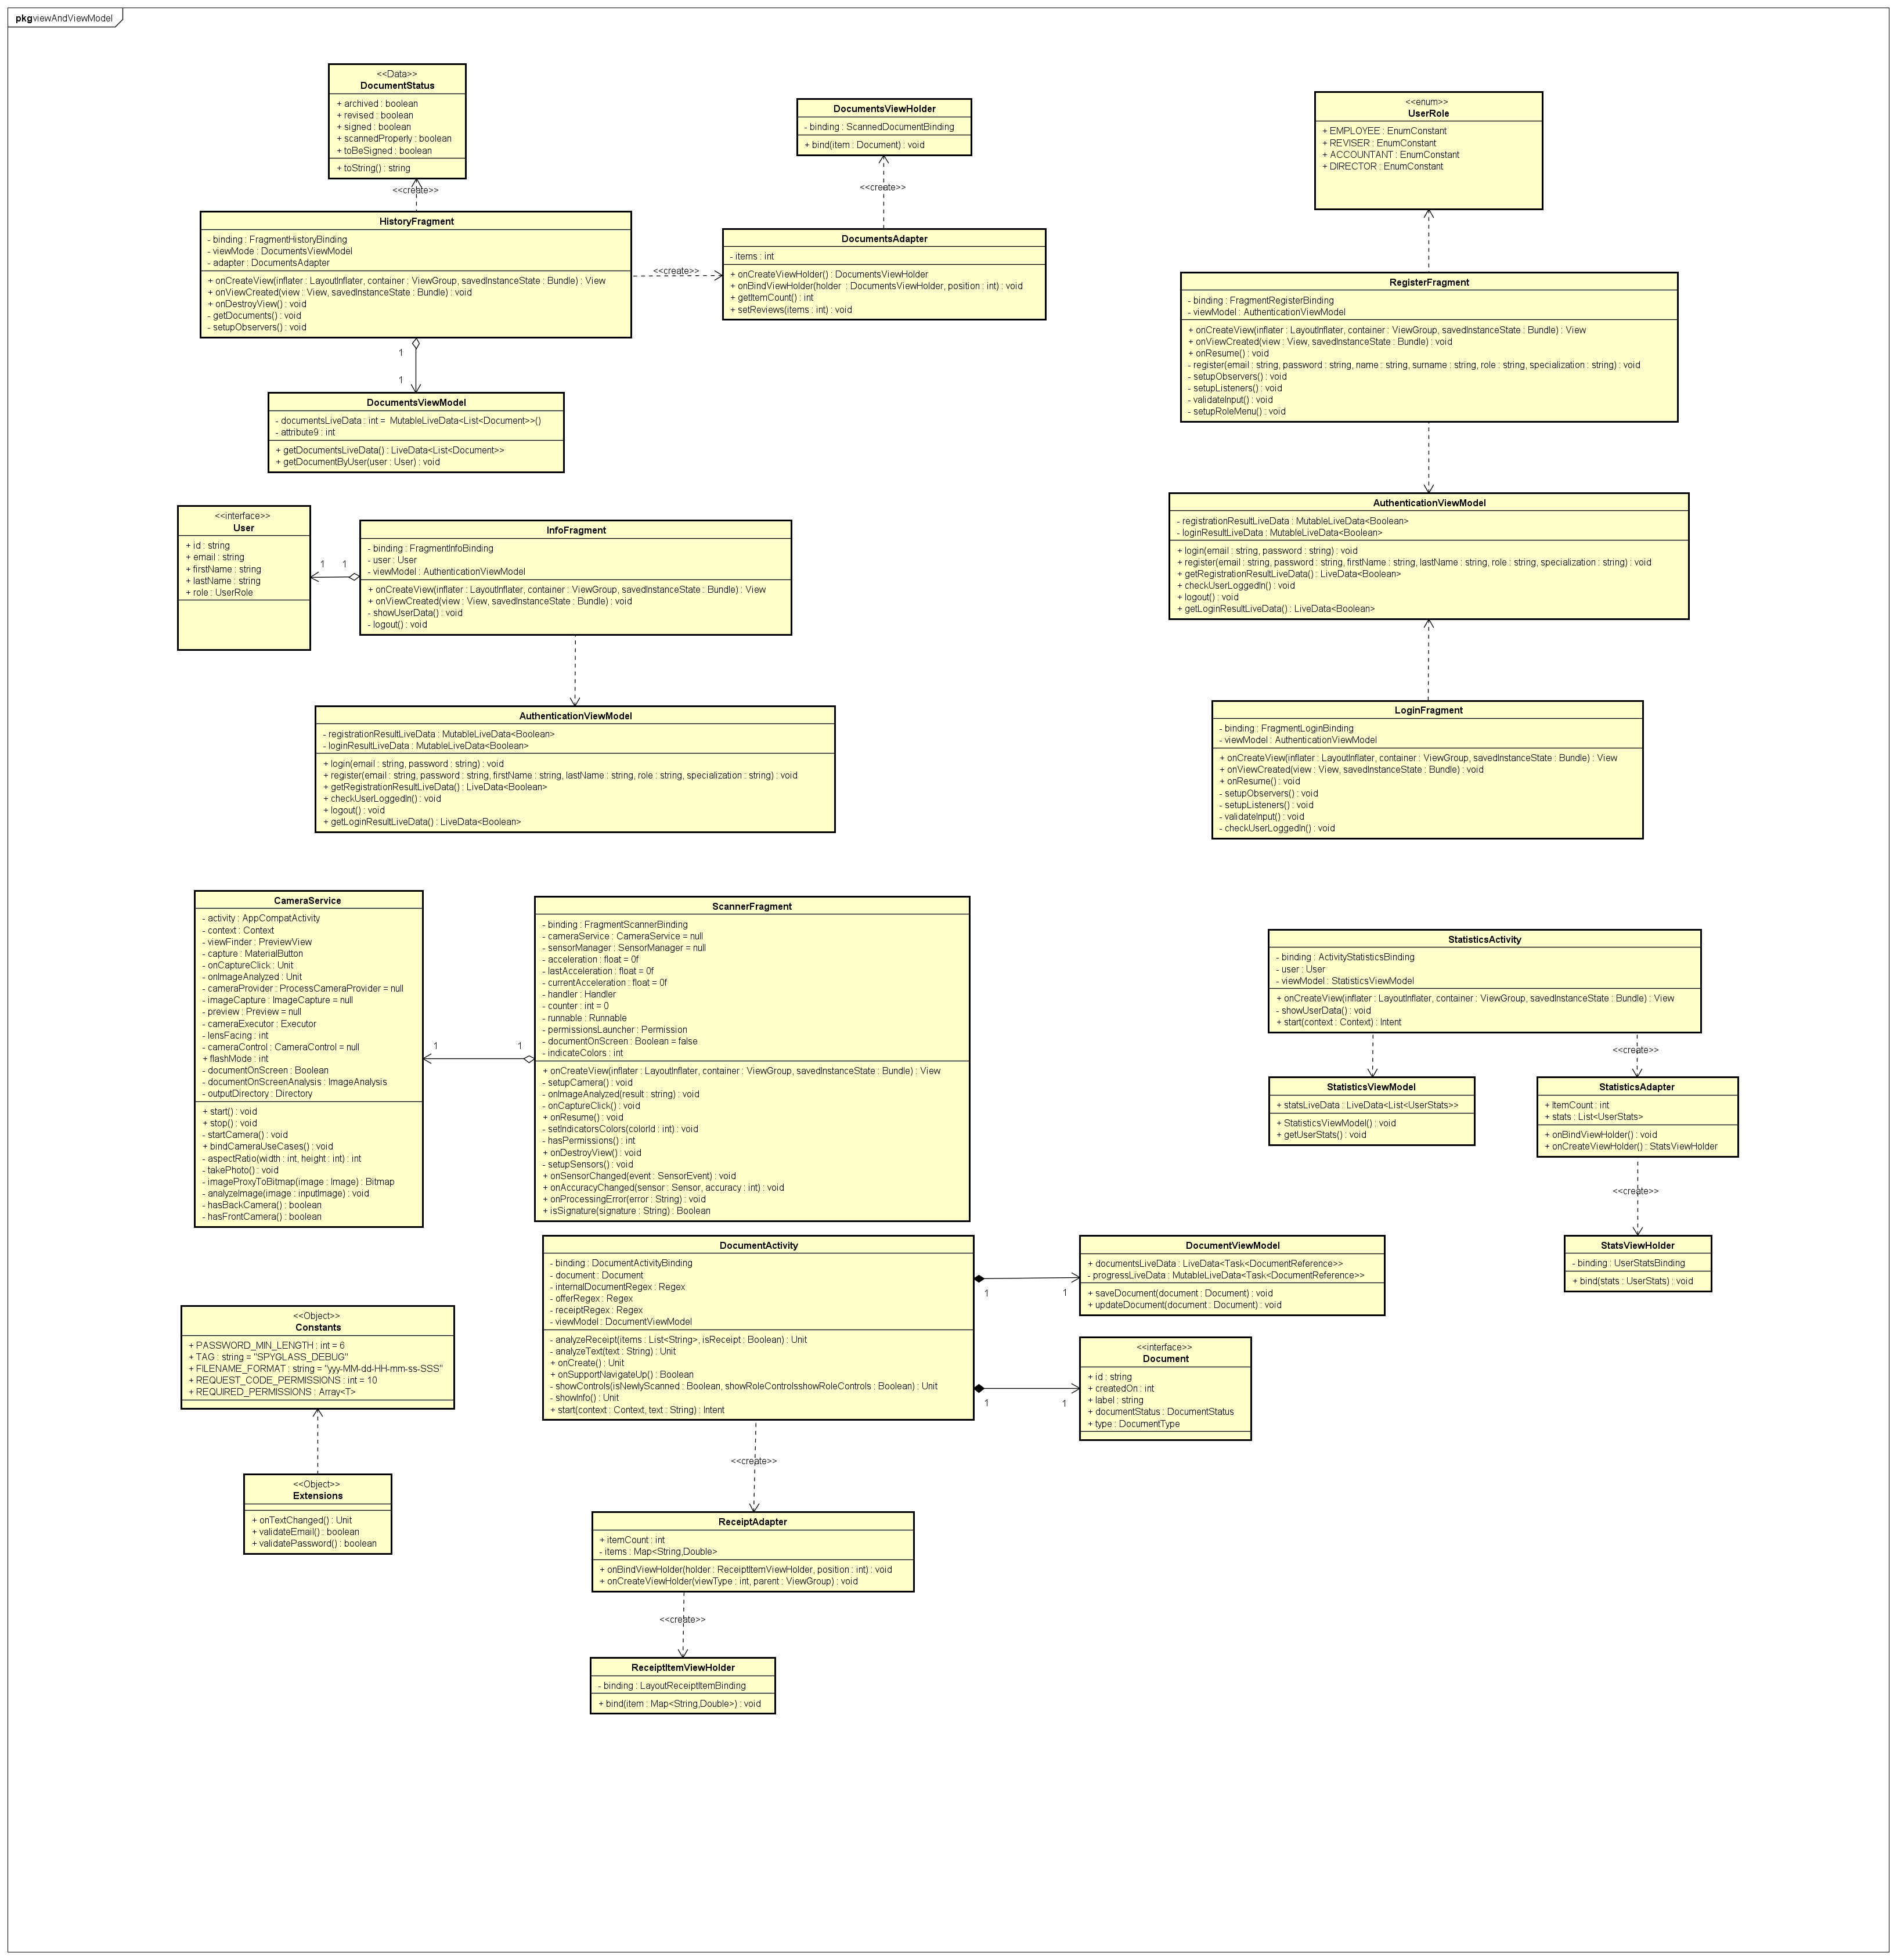
\includegraphics[width=\textwidth]{slike/Dijagram_razreda_viewAndViewModel.png}
				\caption{Dijagram razreda - View s ViewModelom.}
			\end{figure}
		
			\justify{Razredi koji su prikazani na slici 4.6. pripadaju model dijelu arhitekture. Razredi koji predstavljaju vrstu korisnika realiziraju sučelje User, a razredi koji predstavljaju vrstu dokumenta realiziraju sučelje Document.}
			
			\begin{figure}[H]
				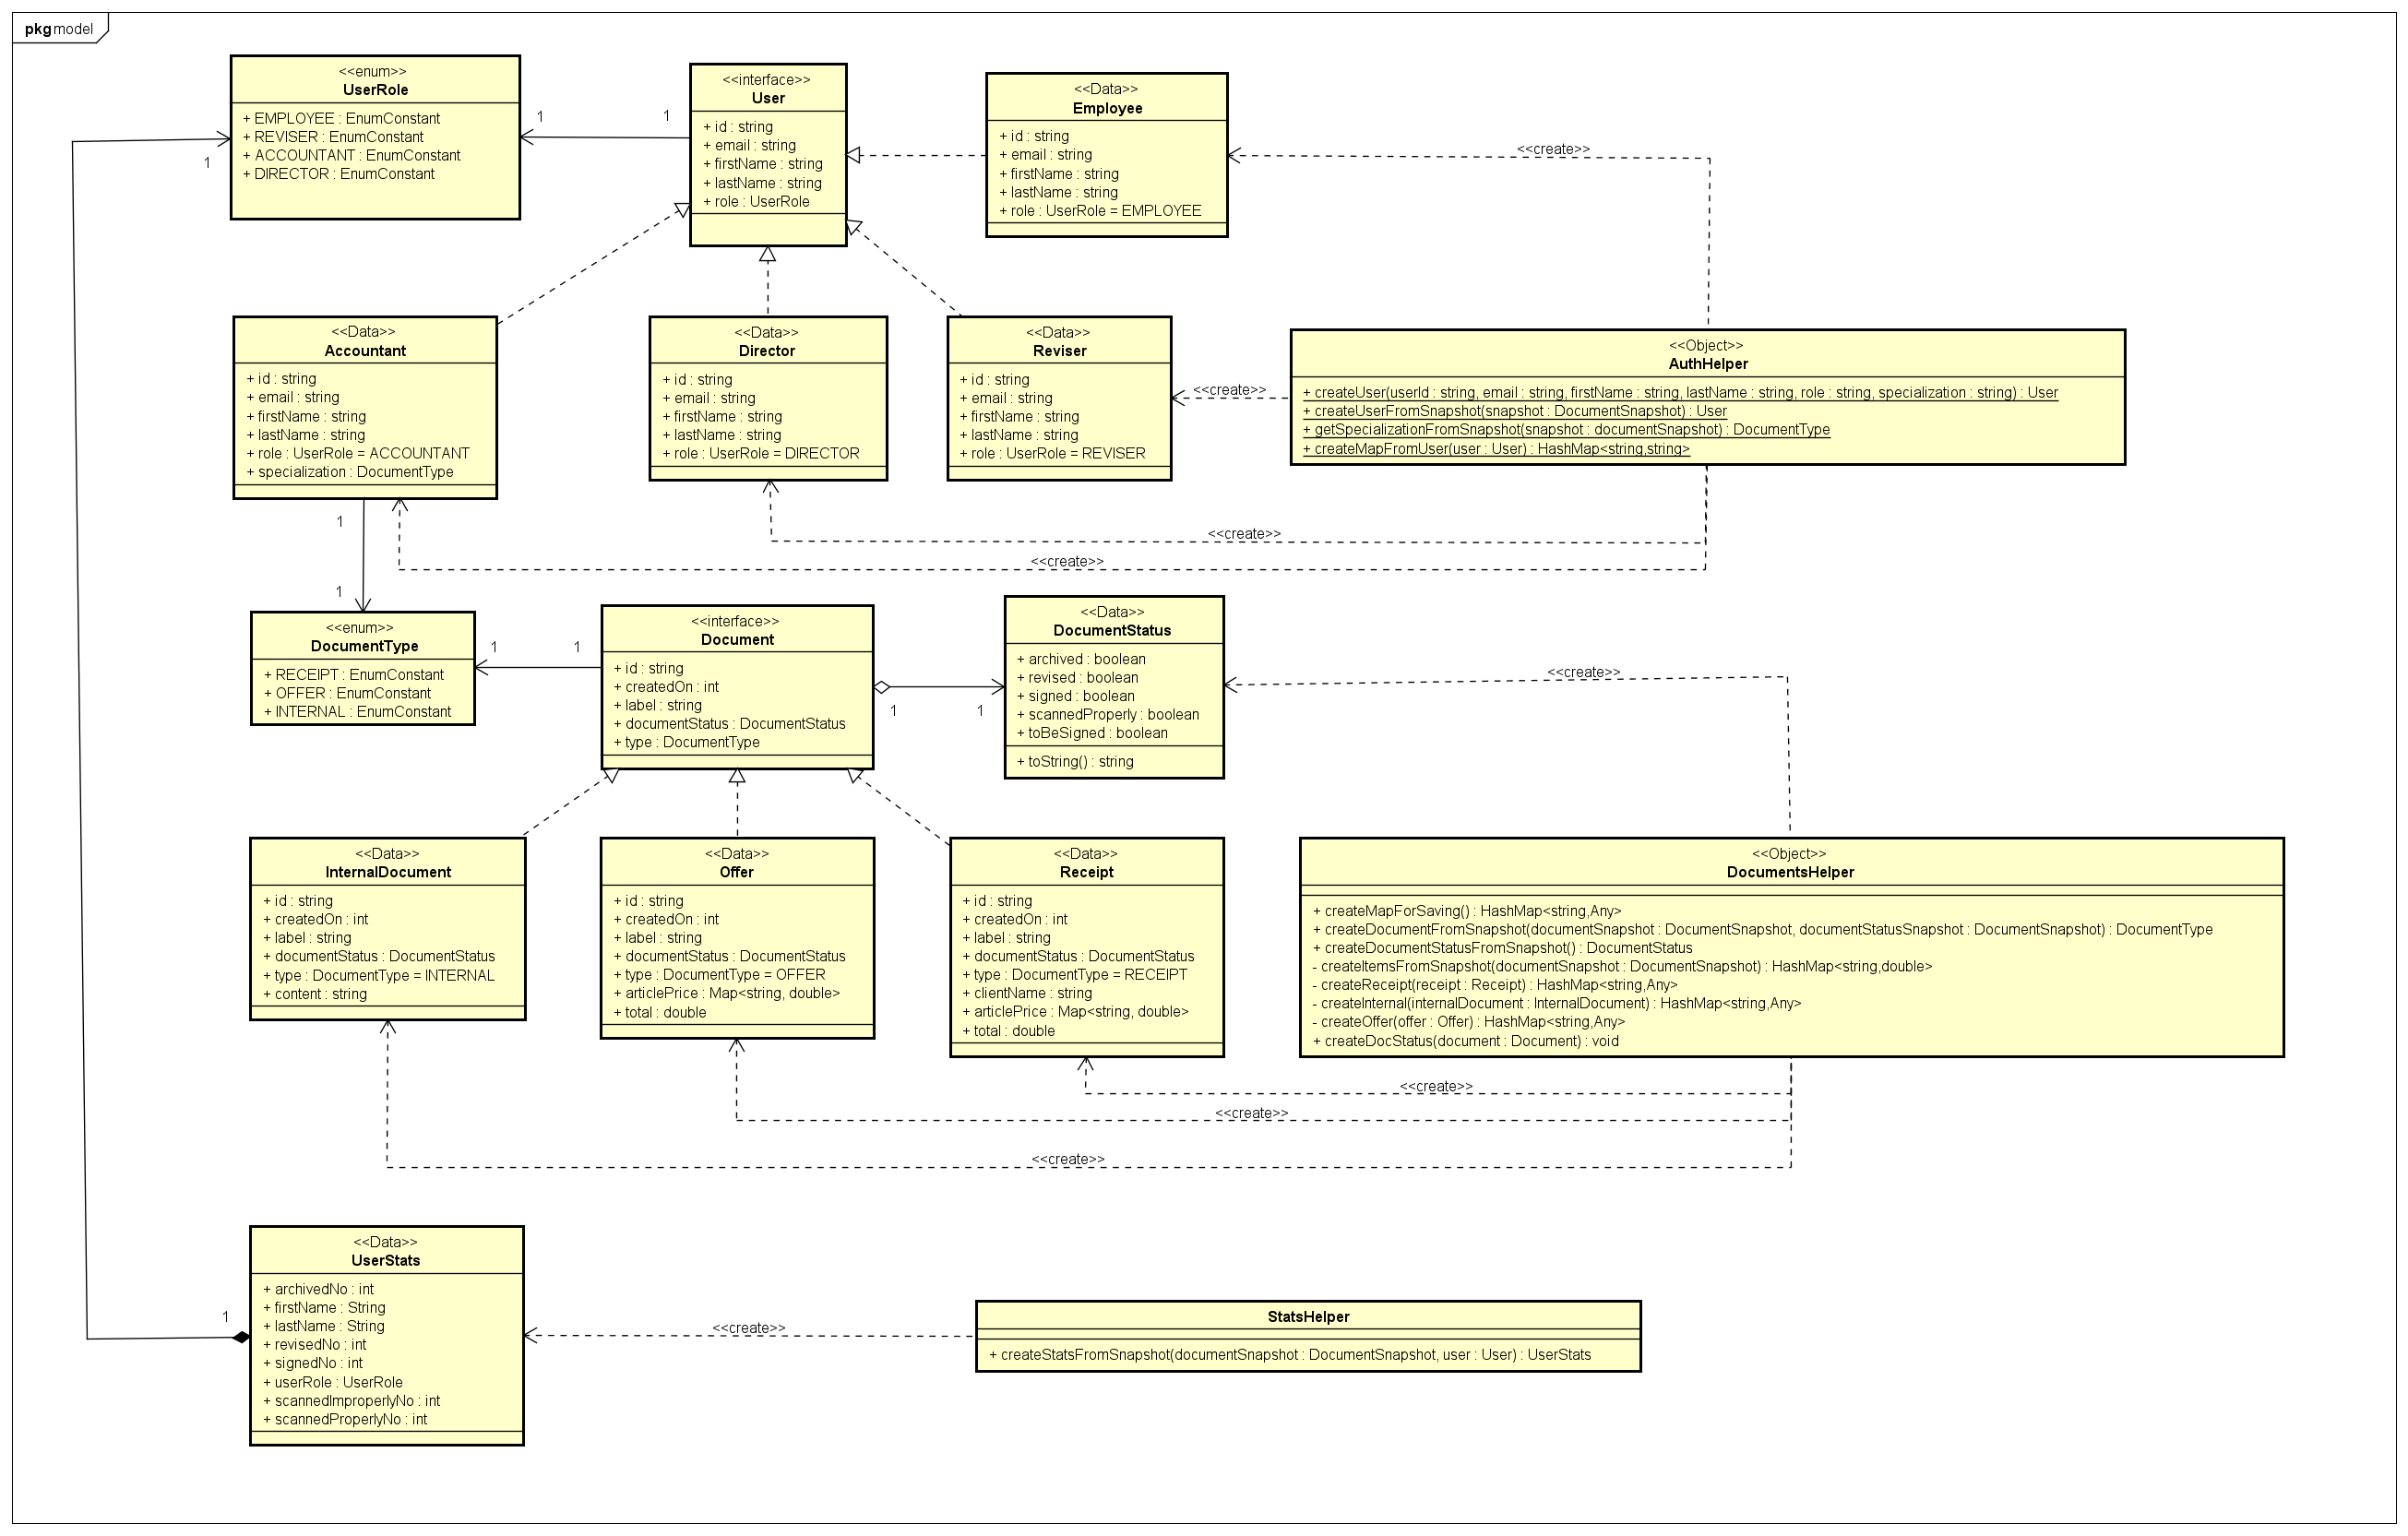
\includegraphics[width=\textwidth]{slike/Dijagram_razreda_model.png}
				\caption{Dijagram razreda - Model}
			\end{figure}
			
			
			\eject
		
		\section{Dijagram stanja}
			
				
			\justify{Dijagram stanja prikazuje stanja objekta te prijelaze iz jednog stanja u drugo temeljene na događajima. Na slici 4.7. prikazan je dijagram stanja za registriranog korisnika, koji može biti direktor, računovođa, revizor ili zaposlenik. Nakon prijave korisnik može skenirati dokument (nakon što akcelerometar i žiroskop to dopuste). Dodirom na gumb za skeniranje otvara se pregled skeniranog dokumenta. Ako korisnik nije zadovoljan skeniranim, ima opciju dodira na gumb \textit{Discard}, a u suprotnom gumb \textit{Save}. Bez obzira koji gumb je dodirnut, aplikacija vraća korisnika na karticu za skeniranje. Dodirom kartice \textit{History} korisniku se prikazuju osobni skenirani dokumenti. Postoji \textit{switch} koji kad se dodirne mijenja prikaz u dokumente koji su potrebni za obrađivanje (revizija, arhiviranje, potpisivanje – ovisno o tipu korisnika). U oba slučaja \textit{switcha} korisnik može dodirom na pojedini dokument vidjeti detalje dokumenta i obaviti akciju. Odlaskom na karticu \textit{Info} prijavljeni korisnik pregledava osobne podatke te ima mogućnost dodirnuti gumb za odjavu ili za prikaz statistike.}
			
			\begin{figure}[H]
				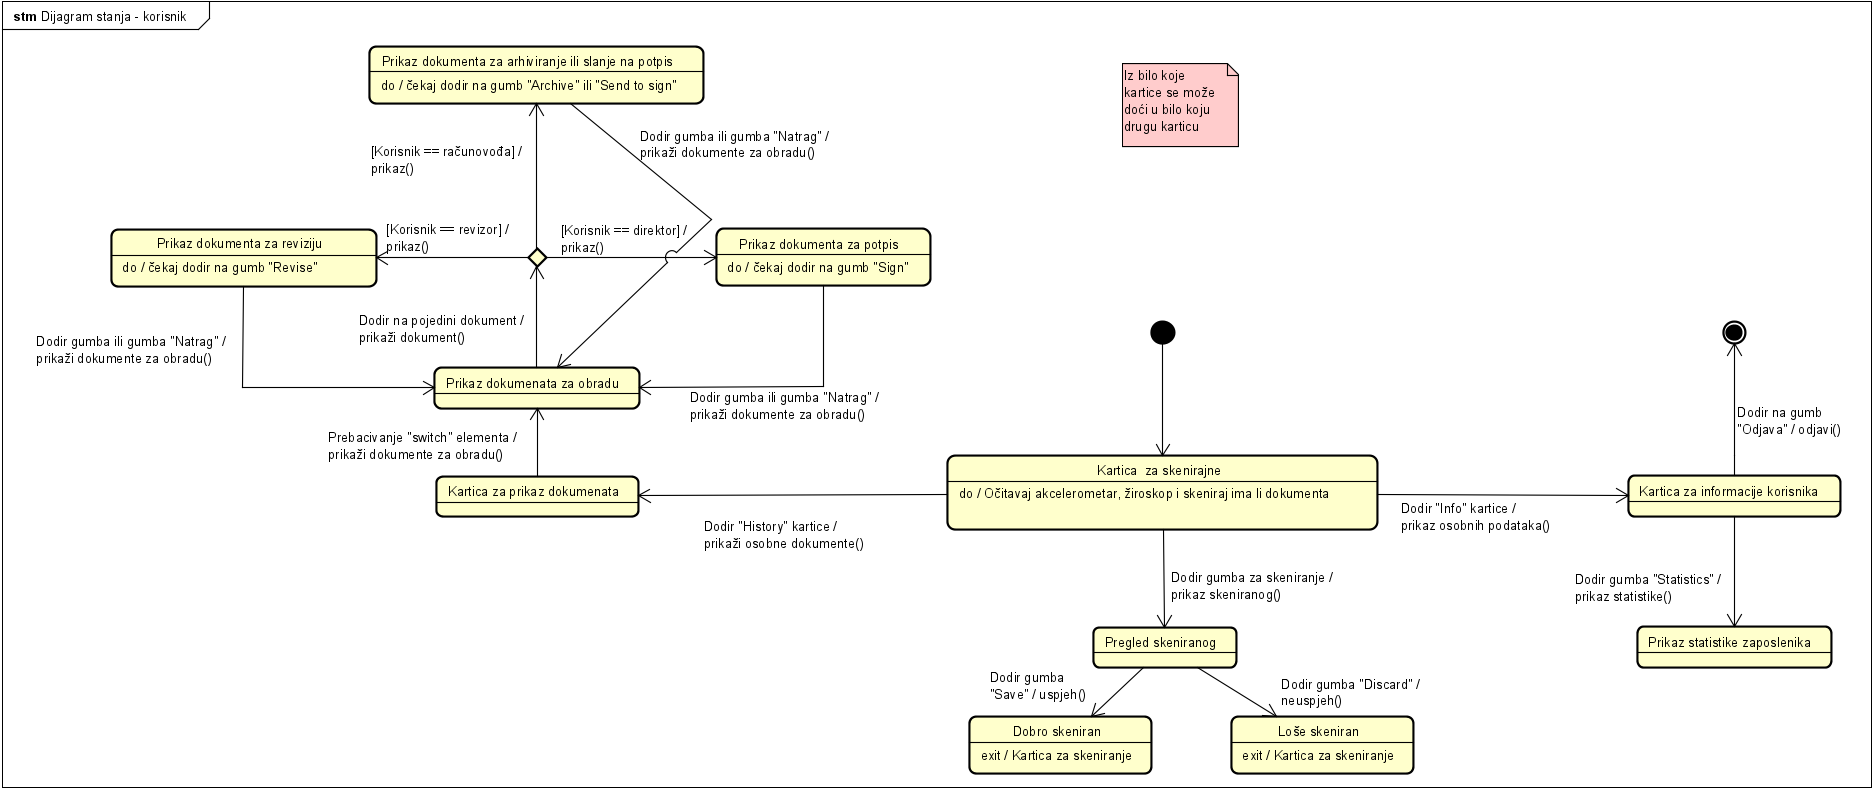
\includegraphics[width=\textwidth]{slike/Dijagram stanja.png}
				\caption{Dijagram stanja - Registrirani korisnik}
			\end{figure}
			
			\eject 
		
		\section{Dijagram aktivnosti}

			
			\justify{Dijagram aktivnosti primjenjuje se za opis modela toka upravljanja ili toka podataka. Na dijagramu aktivnosti prikazan je 
			proces skeniranja dokumenta. Pri modeliranju toka upravljanja svaki novi korak poduzima se nakon završenog prethodnog, osim koraka 
			\textit{Mirovanje od 5 s} i \textit{Detekcija dokumenta}, koji se odvijaju istovremeno. Korisnik se s korisničkim podacima prijavljuje u sustav, 
			skenira željeni dokument, nakon čega mu se prikazuje sažetak dokumenta. Korisnik zatim označava dokument kao dobro ili loše skeniran, 
			dokument se šalje u bazu podataka, te se zajedno s odabirom korisnika pohranjuje u bazu.}
			
			\begin{figure}[H]
				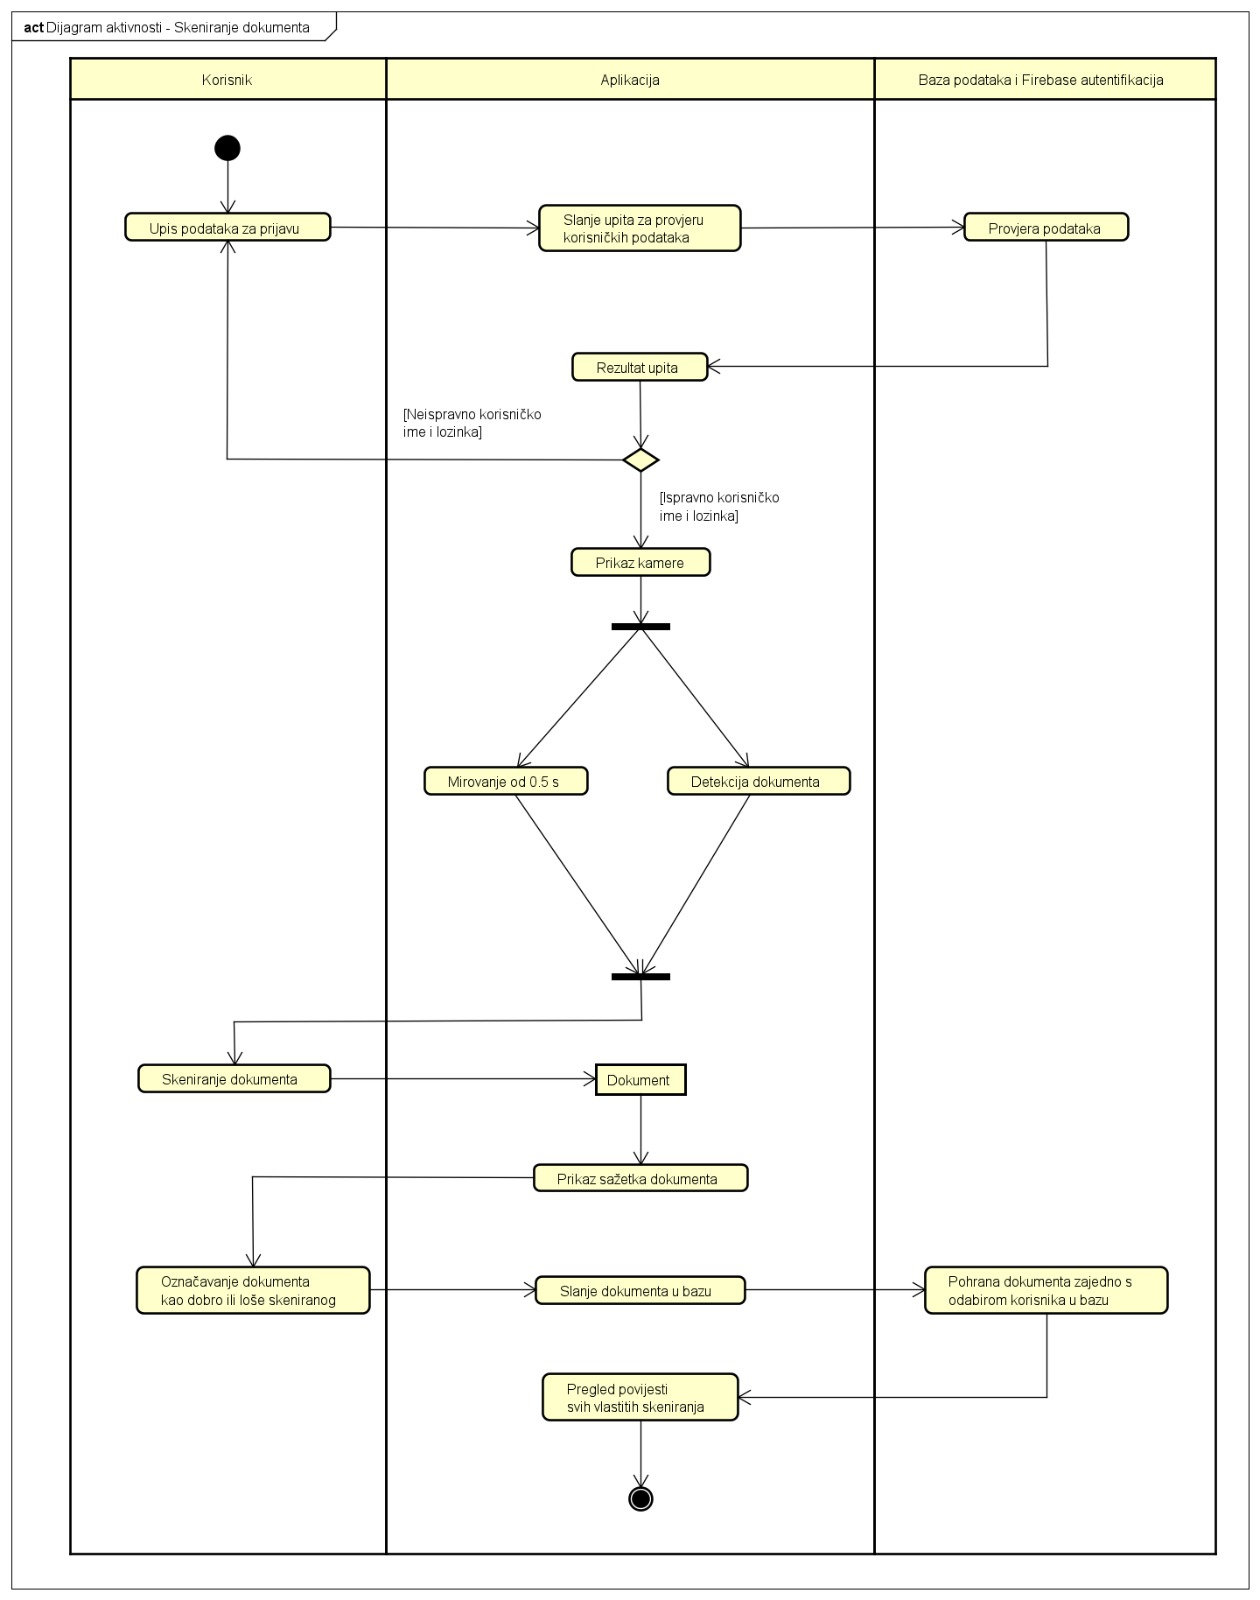
\includegraphics[width=\textwidth]{slike/Dijagram aktivnosti.jpeg}
				\caption{Dijagram aktivnosti - skeniranje dokumenta}
			\end{figure}
			
			\eject
		\section{Dijagram komponenti}
		
			\justify{Dijagram komponenti na slici 4.9. prikazuje unutarnju strukturu aplikacije i komunikaciju s Firebase uslugom koja aplikaciji pruža sve potrebne usluge kao što su NoSQL baza podataka, push obavijesti i autentifikacija korisnika. Aplikacija je modelirana po uzoru na MVVM arhitekturu stoga svako korisničko sučelje ima pripadni model koji njime upravlja. Češće korištene funkcije enkapsulirane su u helper komponente.\par
Prijava i registracija korisnika ostvarena je preko sučelja Auth pomoću Firebase biblioteke za autentifikaciju.\par
Model korisničkog sučelja koristi repozitorij kako bi aplikacija dohvatila ili spremila određene podatke koji se modeliraju pomoću skupa modela za dokumente i korisnike preko sučelja za NoSQL operacije.\par
Skeniranje dokumenata ostvareno je bibliotekom CameraX, a procesiranje skeniranih dokumenata izvodi se interno preko pripadnog sučelja pomoću Google ML Text Recognition biblioteke.\par
Komponenta zadužena za push obavijesti konstantno sluša Firebase dolazne poruke preko sučelja za poruke te ih šalje drugim komponentama aplikacije na prikaz.}
		
			 \begin{figure}[H]
				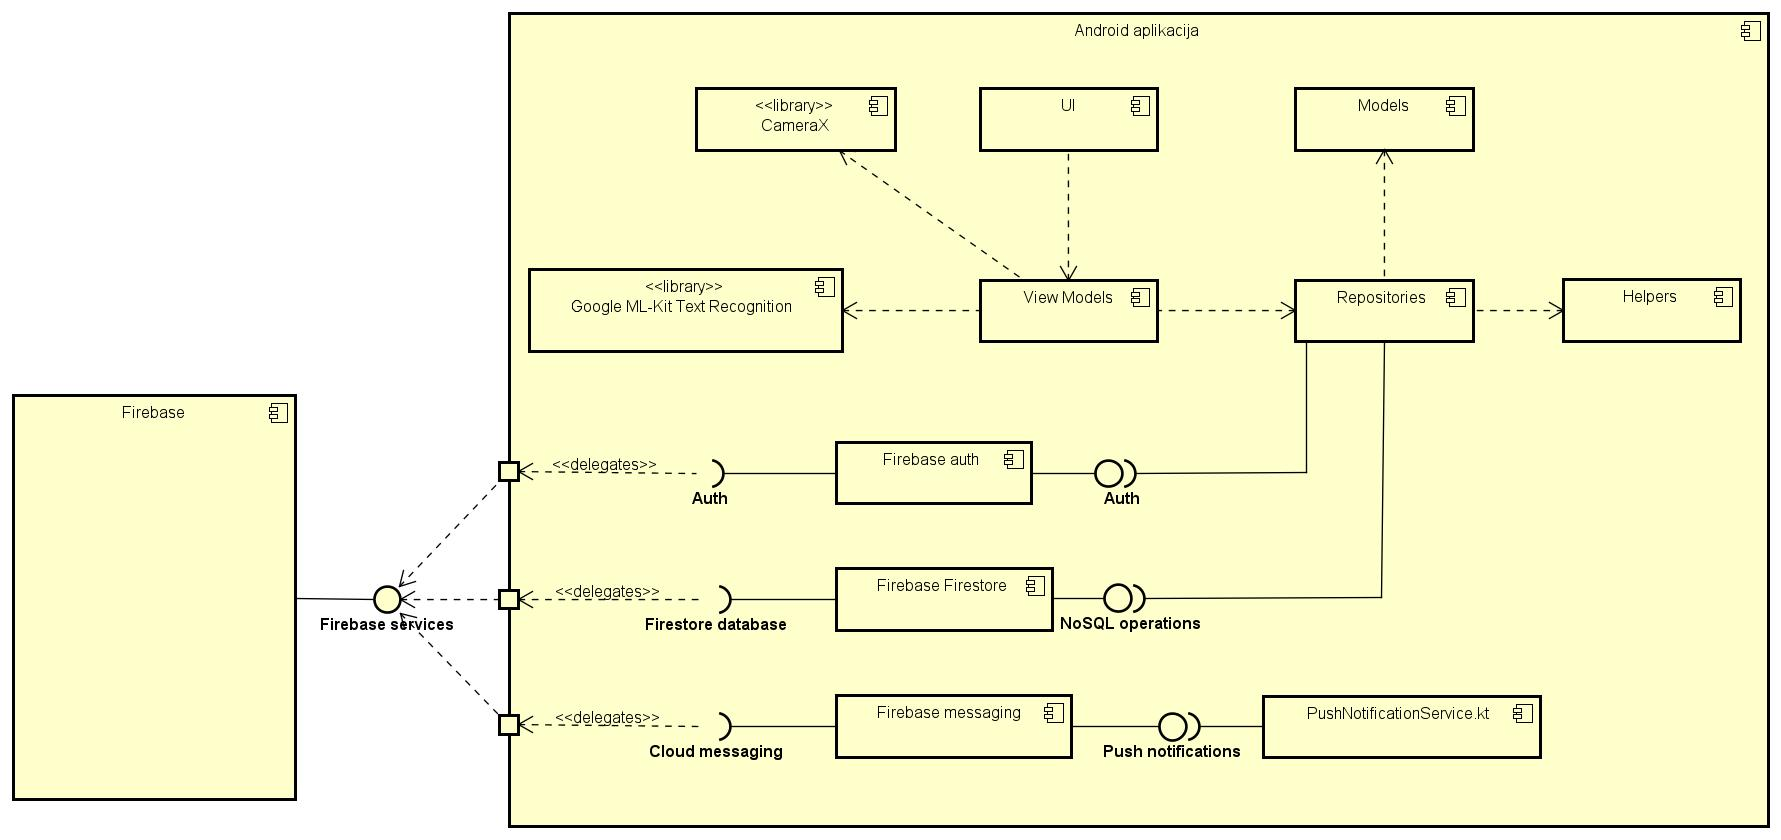
\includegraphics[width=\textwidth]{slike/Dijagram_komponenti.jpg}
				\caption{Dijagram komponenti}
			\end{figure}